\documentclass[11pt,openany]{article}

\input{algebra-preamble}
\usepackage{commath}
\usepackage{caption}
%Tikzpicture
\usepackage{tikz}
\usepackage{tikz-3dplot}
\usepackage{tikz-cd}
\usetikzlibrary{
	3d, % For 3D drawing
	angles,
	arrows,
	arrows.meta,
	backgrounds,
	bending,
	calc,
	decorations.pathmorphing,
	decorations.pathreplacing,
	decorations.markings,
	fit,
	matrix,
	patterns,
	patterns.meta,
	positioning,
	quotes,
	shadows,
	shapes,
	shapes.geometric
}
\input{../preamble/tcolorbox}

\newcommand{\arrowboth}[1][]{\arrow[#1, bend left=15, myarrow]\arrow[bend left=15, myarrow, from=#1]}
\newcommand{\topology}{\mathcal{T}}

\usepackage{multirow}
\usepackage{xcolor,cancel}

\newcommand\hcancel[2][black]{\setbox0=\hbox{$#2$}%
	\rlap{\raisebox{.45\ht0}{\textcolor{#1}{\rule{\wd0}{1pt}}}}#2} 

\setstretch{1.25}
\begin{document}
	\pagenumbering{arabic}
	\begin{center}
		\huge\textbf{Ring Homomorphism $\pi:R\to R/I$}\\
		\vspace{0.5em}
		%	\Large\quad{대수학의 아름다움 서브-스터디}\\
		\vspace{0.5em}
		\normalsize{\today}\\
	\end{center}
	
	\begin{observation*}
		In the ring of integers $\Z$, there are three ideals containing $4\Z$: \[
		4\Z\subset 2\Z \subset\Z.
		\] In the ring $\Z/4\Z$, there are three ideals total: \begin{align*}
			\gen{0}&=\set{0\cdot x:x\in\Z/4\Z}=\set{0},\\
			\gen{1}&=\set{1\cdot x:x\in\Z/4\Z}=\set{0,1,2,3}=\gen{3}\ \text{and} \\
			\gen{2}&=\set{2\cdot x:x\in\Z/4\Z}=\set{0,2}.
		\end{align*}
		\begin{center}
			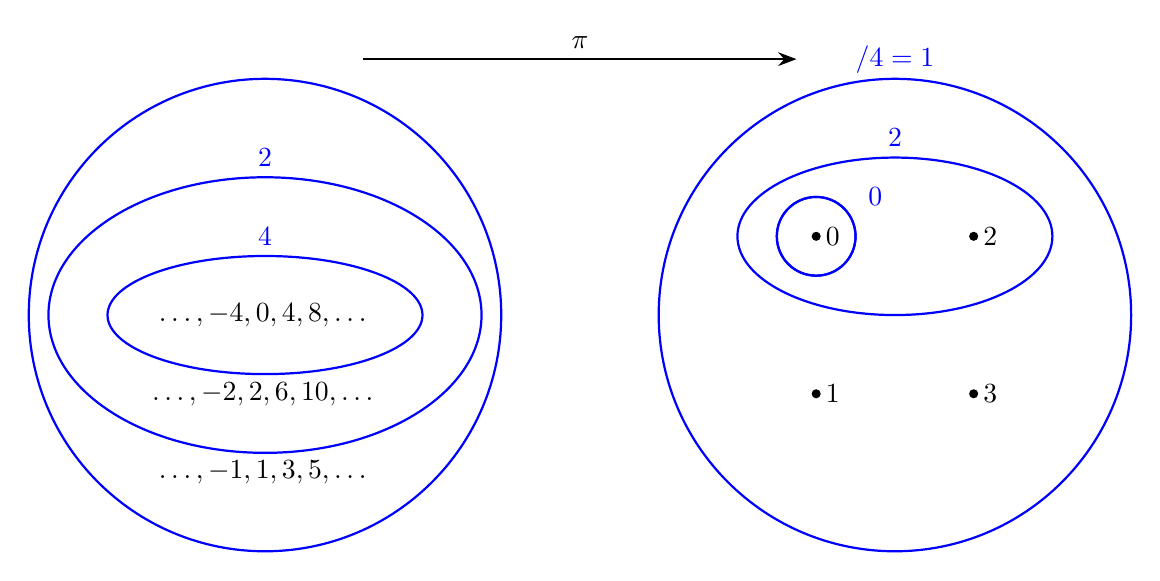
\begin{tikzpicture}
				% Draw the sets A and B
				\draw[thick, color=blue] (-4,0) ellipse (3 and 3);
				\draw[thick, color=blue] (-4,0) ellipse (2 and .75);
				\draw[thick, color=blue] (-4,0) ellipse (2.75 and 1.75);
				\draw[thick, color=blue] (4,0) ellipse (3 and 3);
				
				% Labels for sets
				\node at (-4, 3.25) {$\textcolor{blue}{\Z}$};
				\node at (-4, 2) {$\textcolor{blue}{2\Z}$};
				\node at (-4, 1) {$\textcolor{blue}{4\Z}$};
				\node at (4, 3.25) {$\textcolor{blue}{\Z/4\Z=\gen{1}}$};
				
				\node at (-4, 0) {$\dots,-4,0,4,8,\dots$};
				\node at (-4, -1) {$\dots,-2,2,6,10,\dots$};
				\node at (-4, -2) {$\dots,-1,1,3,5,\dots$};
				
				% Draw the arrows representing the function
				\draw[-Stealth, thick] (-2.75, 3.25) -- (2.75,3.25) node[midway, above] {$\pi$};
				
				\draw[fill] (3,1) circle (.05) node[right] {0};
				\draw[fill] (5,1) circle (.05) node[right] {2};
				\draw[fill] (3,-1) circle (.05) node[right] {1};
				\draw[fill] (5,-1) circle (.05) node[right] {3};
				
				
				\draw[thick, color=blue] (3,1) circle (.5);
				\draw[thick, color=blue] (4,1) ellipse (2 and 1);
				\draw[thick, color=blue] (3,1) circle (.5);
				
				\node at (4, 2.25) {$\textcolor{blue}{\gen{2}}$};
				\node at (3.75, 1.5) {$\textcolor{blue}{\gen{0}}$};
			\end{tikzpicture}
		\end{center} Here, there is a bijection $\set{4\Z,2\Z,\Z}\to\set{\gen{0},\gen{1},\gen{2}}$.
	\end{observation*}
	
	\newpage
	\begin{itemize}
		\item Let $R$ be a ring, and $I\subseteq R$ be an ideal.
		\item We writes ``$I\lhd R$'' to indicate that $I$ is an ideal of $R$.
		\item The natural projection map is \[
		\fullfunction{\pi}{R}{R/I}{r}{r + I}
		\] for all $r\in R$.
		\item Let \[
		\mathcal{L}_I(R):=\set{J\subseteq R:I\subseteq J\ \text{and}\ J\lhd R}
		\] is the set of ideals of $R$ that contain $I$, and let \[
		\mathcal{L}(R/I):=\set{K\subseteq R/I: K\lhd R/I}
		\] is the set of ideals of the quotient ring $R/I$.
	\end{itemize}
	\begin{center}
		\begin{tikzpicture}
			% Draw the sets A and B
			\draw[thick] (-4,0) ellipse (3 and 3);
			\draw[thick] (-4,1) ellipse (1.5 and 1.5);
			\draw[thick] (-5,-.5) ellipse (1.5 and 1.5);
			\draw[thick] (-3,-.5) ellipse (1.5 and 1.5);
			
			\draw[thick] (4,0) ellipse (3 and 3);
			
			% Labels for sets
			\node at (-4, 3.25) {$R$};
			\node at (-4, 2) {$J_1\lhd R$};
			\node at (-5.5, -1.25) {$J_2\lhd R$};
			\node at (-2.5, -1.25) {$J_3\lhd R$};
			\node at (4, 3.25) {$R/I$};
			
			\node at (-4, 0) {\textcolor{red}{$I$}};
			
			% Draw the arrows representing the function
			\draw[-Stealth, thick] (-2.75, 3.25) -- (2.75,3.25) node[midway, above] {$\pi$};
			
			\draw[thick] (4,1) circle (1.5);
			\draw[thick] (3,-.5) circle (1.5);
			\draw[thick] (5,-.5) circle (1.5);
			
			\node at (4,2) {$K_1\lhd R/I$};
			\node at (2.5,-1) {$K_2\lhd R/I$};
			\node at (5.5,-1) {$K_3\lhd R/I$};
		\end{tikzpicture}
	\end{center}
	
	\thmbox{
		\begin{theorem*}
			There is a one-to-one correspondence between the set of  ideals of $R$ containing $I$ and the set of ideals of $R/I$. That is, there is a bijection \[
			\phi:\mathcal{L}_I(R)\to\mathcal{L}(R/I).
			\]
	\end{theorem*}}
	\begin{proof}
		Consider \[
		\fullfunction{\phi}{\mathcal{L}_I(R)}{\mathcal{L}(R/I)}{J}{J/I}
		\] and \[
		\fullfunction{\psi}{\mathcal{L}(R/I)}{\mathcal{L}_I(R)}{K}{\pi^{-1}[K]=\set{r\in R:r+I\in K}}.
		\] We must show that \begin{itemize}
			\item $\psi[\phi[J]]=J$ for all $J\subseteq R$ s.t. $I\subseteq J$;
			\item $\phi[\psi[K]]=K$ for all $K\subseteq R/I$.
		\end{itemize}
		\begin{enumerate}[(i)]
			\item Let $J\in\mathcal{L}_I(R)$, \ie, $I\subseteq J\subseteq R$ and $J\lhd R$. Then \begin{align*}
				\phi[J] &= J/I=\set{r+I:r\in J},	
			\end{align*} and so \begin{align*}
				\psi[\phi[J]] &= \psi[J/I]\\
				&=\set{r\in R:r+I\in J/I},\\
				&=\set{r\in R:r\in J},\\
				&= J.
			\end{align*}
			\item Let $K\in\mathcal{L}(R/I)$, \ie, $K\subseteq R/I$ and $K\lhd R/I$. Then \begin{align*}
				\psi[K] &= \pi^{-1}[K]=\set{r\in R:r+I\in K},	
			\end{align*} and so \begin{align*}
				\phi[\psi[K]] &= \phi[\pi^{-1}[K]]\\
				&=\set{r+I:r+\pi^{-1}[K]},\\
				&=\set{r+I:r+I\in K},\\
				&= K.
			\end{align*}
		\end{enumerate}
	\end{proof}
\end{document}
